% !TEX program = xelatex
\documentclass[fontsize=14pt,a4paper]{scrartcl}
\usepackage[english,russian]{babel} 
\usepackage{fontspec} 
\defaultfontfeatures{Ligatures={TeX},Renderer=Basic} 
\setmainfont[Ligatures=TeX]{PT Astra Serif}

\usepackage{unicode-math}
\unimathsetup{math-style=TeX}
\setmathfont{Cambria Math}
\setmathfont[range=\mathup/{num}]{Times New Roman}
\setmathfont[range=\mathit/{greek,Greek,latin,Latin,Cyrillic,cyrillic}]{Cambria Math}
\setmathfont[range=\mathup/{greek,Greek,latin,Latin,Cyrillic,cyrillic}]{Cambria Math}
\setmathfont[range={"2212,"002B,"003D,"0028,"0029,"005B,
"005D,"221A,"2211,"2248,"222B,"007C,"2026,"2202,"00D7,"0302,
"2261,"0025,"22C5,"00B1,"2194,"21D4}]{Cambria Math}
\setmathfont[version=bold,FakeBold=3]{Cambria Math}

\usepackage{indentfirst}
\usepackage{graphicx}
\usepackage{amsmath}
\usepackage{float}

\usepackage{pgfplots}
\usepackage{pgfplotstable}

\def\arraystretch{1.3}%

\usepackage[left=20mm, top=20mm, right=10mm, bottom=20mm, nohead, footskip=10mm]{geometry}
\begin{document}
  \begin{titlepage}                                                         
    \newpage                                                                        
    \begin{center}   
      Министерство образования и науки Российской Федерации  \\ 
      \vspace{1em}                                                    
      {\mdseries
        Федеральное государственное бюджетное образовательное \\
        учреждение высшего образования \\
        «ОМСКИЙ ГОСУДАРСТВЕННЫЙ ТЕХНИЧЕСКИЙ УНИВЕРСИТЕТ»
      }                               
      \vspace{1em}      

      {\bfseries Кафедра «Средства связи и информационная безопасность»}  

      \vspace{\fill}                                                         
                                   
      {\bfseries ОТЧЕТ } \\                                 
      По дисциплине «Электродинамика и распространение радиоволн» \\ 
      \vspace{1em} 
      Практическая работа №5 \\                                                           
    \end{center}                                                          
                                                                                        
    \vspace{\fill}                                                         
                                                                                        
    \hfill\parbox{5cm}{
      Выполнил\\
      студент гр. ЗИС-231:\\
      Белый В.Е. \\
      \\
      Проверил:\\
      проф., д.н. \\
      Богачков И.В.\\
    }                                                                                                                              
                                                                                                                                                                              
    \vspace{\fill}                                                    
                                                                                        
    \begin{center}                                                        
    Омск 2020                                                                
    \end{center}                                                          
                                                                                        
    \end{titlepage}

    \newpage
    {\bfseries Задание 5.} 
    Спроектировать коаксиальную, двухпроводную, симметричную полосковую и микрополосковую линии на заданное $Z_c$ с поперечным размером не более $d_{max}$ при параметрах диэлектрика $\varepsilon$ и $tg\delta$. Материал проводников – медь, рабочая частота $f$. 
    Найти основные характеристики ЛП. Найти затухание по амплитуде и по мощности отрезка спроектированных ЛП длиной $l$. Произвести сравнительный анализ.

    \begin{table}[h]
      \begin{center}
        \label{tab:table1}
        \pgfplotstabletypeset[
          column type=l,
          before row=\hline,every last row/.style={after row=\hline},
          columns/v/.style={
            column type=|l|,
            column name={Вариант},
          },
          columns/z/.style={
            column type=l|,
            column name={$Z_c, \; \text{Ом}$},
          },
          columns/e/.style={
            column type=l|,
            column name={$\varepsilon$},
          },
          columns/tg/.style={
            column type=l|,
            column name={$tg\delta, \times 10^{-4}$},
          },
          columns/d/.style={
            column type=l|,
            column name={$d_{max}, \; \text{мм}$},
          },
          columns/l/.style={
            column type=l|,
            column name={$l, \; \text{м}$},
          },
          columns/f/.style={
            column type=l|,
            column name={$f, \; \text{МГц}$},
          },
          columns/mu/.style={
            column type=l|,
            column name={$\mu$},
          },
          col sep=semicolon,
          /pgf/number format/read comma as period
        ]{data/source.csv}
        \caption{Исходные данные.}
      \end{center} 
    \end{table}

    {\bfseries Решение:}\\ 
    \indent Спроектируем коаксиальную линию передачи (КЛ):

    \begin{figure}[H]
      \centering
      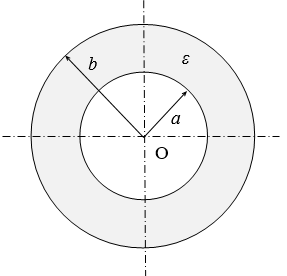
\includegraphics[scale=0.8]{data/fig/1.png}
      \caption{Поперечное сечение КЛ}
      \label{fig:ris1}
    \end{figure}

    \indent Рассчитаем размеры КЛ:

    \begin{equation}
      Z_C=60\sqrt{\frac{\mu}{\varepsilon}}\ln{\frac{b}{a}}
    \end{equation}

    \begin{equation}
      \ln{\frac{b}{a}}=\frac{Z_C}{60\sqrt{\frac{\mu}{\varepsilon}}}=4,95    \frac{\ b}{a}=2.428
    \end{equation}

    \begin{equation}
      2b+1=d_{max}
    \end{equation}

    \begin{equation}
      b=\frac{d_{max}-1}{2}=3\; \text{мм}; \; a=\frac{b}{2.427}=0,021\; \text{мм};
    \end{equation}

    \indent Рассчитаем погонные индуктивность и емкость ЛП:
    \begin{equation}
      L_0=\frac{\mu_0\mu_1}{\pi}\ln{\frac{\ D}{a}=1.77\cdot {10}^{-7}} \text{Гн/м};
    \end{equation}

    \begin{equation}
      C_0=\frac{\varepsilon_a2\pi}{ln\frac{b}{a}}=6.27\cdot 10^{-10} \text{Ф/м}
    \end{equation}

    \indent Постоянная фазы:
    \begin{equation}
      \beta_0=\omega\sqrt{L_0C_0}=106.05
    \end{equation}

    Рассчитаем коэффициенты затухания в проводнике и диэлектрике:
    \begin{equation}
      \alpha_\text{пр}=\frac{\sqrt{\pi f\mu_0\mu}}{4\pi Z_c \sqrt\sigma}\cdot\left(\frac{\mathrm{1}}{\mathrm{a}}\mathrm{+} \frac{\mathrm{1} }{\mathrm{b}}\right)\mathrm{=4.121*}{\mathrm{10}}^{\mathrm{-3}}
    \end{equation}

    Т.к $\alpha_\text{изл}=0$, то коэффициент затухания в ЛП:
    \begin{equation}
      a_\text{д}=\frac{\beta_0}{2}\left(tg\delta_\text{пол}+\frac{\sigma}{\omega\varepsilon_\alpha}\right)=1,386*10^{10} \; \text{1/м};
    \end{equation}
    \begin{equation}
      \alpha=\alpha_\text{пр}+\alpha_\text{д}+\alpha_\text{изл}=0.012 \; \text{1/м};
    \end{equation}

    Рассчитаем затухание по амплитуде и мощности:
    \begin{equation}
      A=\exp{\left(\alpha z\right)}=1.032
    \end{equation}
    \begin{equation}
      A_\alpha=\exp{\left(2\alpha z\right)}=1,049
    \end{equation}

    Рассчитаем максимальное напряжение и мощность ЛП ($E_\textup{проб}^2=30 \; \text{кВ/см}$):
    \begin{equation}
      P_{max}=\frac{\pi a^2}{Z_c}\cdot\ln{\left(\frac{b}{a}\right)}\cdot E_\text{проб}^2=17 \; \text{МВт}
    \end{equation}

    \begin{equation}
      U_{max}=\sqrt{P_{max}Z_c}=27,658 \; \text{кВ}
    \end{equation}
\\
    \indent Спроектируем двухпроводную линию передачи (ДЛ):
    \begin{figure}[H]
      \centering
      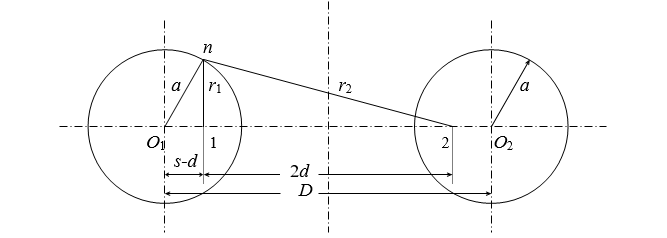
\includegraphics[scale=0.95]{data/fig/2.png}
      \caption{Поперечное сечение двухпроводной линии}
      \label{fig:ris2}
    \end{figure}

    \indent Рассчитаем размеры линии:
    \[
      \begin{cases}
        120\sqrt{\frac{\mu}{\varepsilon}}ln\left(\frac{0,5D}{a} + \sqrt{\left(\frac{0,5D}{a}\right)^2 -1}\right) = Z_c\\
        2a+D=d_{max}
      \end{cases}
    \]
    \[a=5,754\; \text{мм}; \; D=12,492\;\text{мм};\]

    Рассчитаем постоянную фазы:
    \begin{equation}
    \beta_0=\omega\sqrt{L_0C_0}=5,054
    \end{equation}

    Рассчитаем коэффициенты затухания в проводнике и диэлектрике:
    \begin{equation}
      \alpha_\text{пр}=\frac{\sqrt{\pi f\mu_0}}{4\pi Z_C}\cdot\frac{\sqrt\mu}{\sqrt\sigma}\cdot\frac{D}{\sqrt{D^2-4a^2}}=1,472 \cdot {10}^{-5} \; \text{1/м};
    \end{equation}
    \begin{equation}
      \alpha_\text{д}=\frac{\beta_0}{2}\left(tg\delta_\text{пол}+\frac{\sigma}{\omega\varepsilon_\alpha}\right)=5,753 \cdot {10}^{5} \; \text{1/м};
    \end{equation}

    Т.к $\alpha_\text{изл}=0$, то коэффициент затухания в ДЛ:
    \begin{equation}
      \alpha=\alpha_\text{пр}+\alpha_\text{д}+\alpha_\text{изл}=5,753 \cdot {10}^{5} \; \text{1/м}; 
    \end{equation}

    По условию проводник изготовлен из меди, тогда $\mu=1$ и погонная индуктивность двухпроводной линии:
    \begin{equation}
      L_0=\frac{\mu_0}{\pi}\left(ln{\frac{D}{a}}+\frac{1}{4}\right) = 3,538\cdot 10^{-7} \; \text{Гн/м};
    \end{equation}

    Воспользуемся теоремой Аполония для определения положения электрических осей относительно геометрических (рис. \ref{fig:ris2}):
    \[
      \begin{cases}
        (s-d)(s+d)=a^2\\
        2s=D
      \end{cases}
    \]
    \[d=2,43\;\text{мм}; \; s=6,246\;\text{мм};\]

    Т.к расстояние $D$ сравнимо с радиусом проводника $a$ электрические оси проводов должны быть смещены относительно геометрических осей на некоторое расстояние $(s-d)$ и тогда погонная емкость двухпроводной линии:
    \begin{equation}
      C_0=\frac{\pi\varepsilon\varepsilon_0}{ln{\left(\frac{D-(s-d)}{a}\right)}}=8,128\cdot 10^{-11} \; \text{Ф/м};
    \end{equation}
    Рассчитаем максимальное напряжение и мощность ДЛ ($E_\textup{проб}^2=30 \; \text{кВ/см}$):
    \begin{equation}
      U_{max}=a \sqrt{2}\sqrt{\frac{D-2a}{D+2a}}\ln{\frac{D}{a}}E_\text{проб}=3,83\cdot 10^6 \; \text{В};
    \end{equation}
    \begin{equation}
      P_{max}=\frac{U^2_{max}}{Z_c}=3,259\cdot 10^{11} \; \text{Вт};
    \end{equation}

    \begin{figure}[h!]
      \centering
      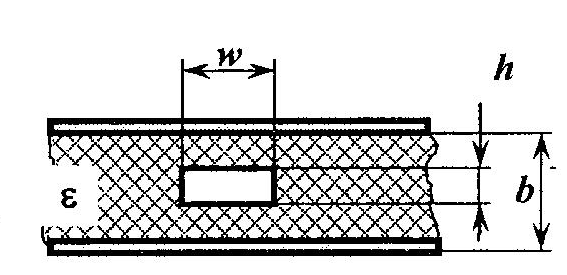
\includegraphics[scale=0.5]{data/fig/3.png}
      \caption{Сечение СПЛ}
      \label{fig:ris3}
    \end{figure}

    \begin{figure}[h!]
      \centering
      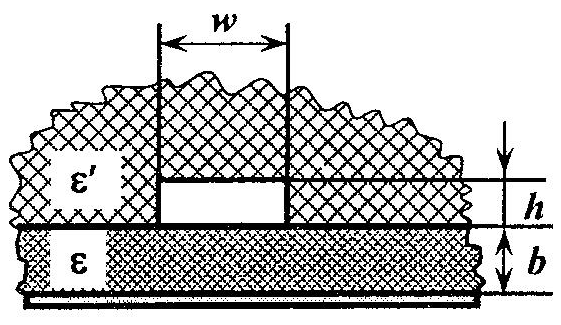
\includegraphics[scale=0.5]{data/fig/4.png}
      \caption{Сечение МПЛ}
      \label{fig:ris4}
    \end{figure}
\end{document}